\section{Combining Learning and Control}
% \begin{figure}
% 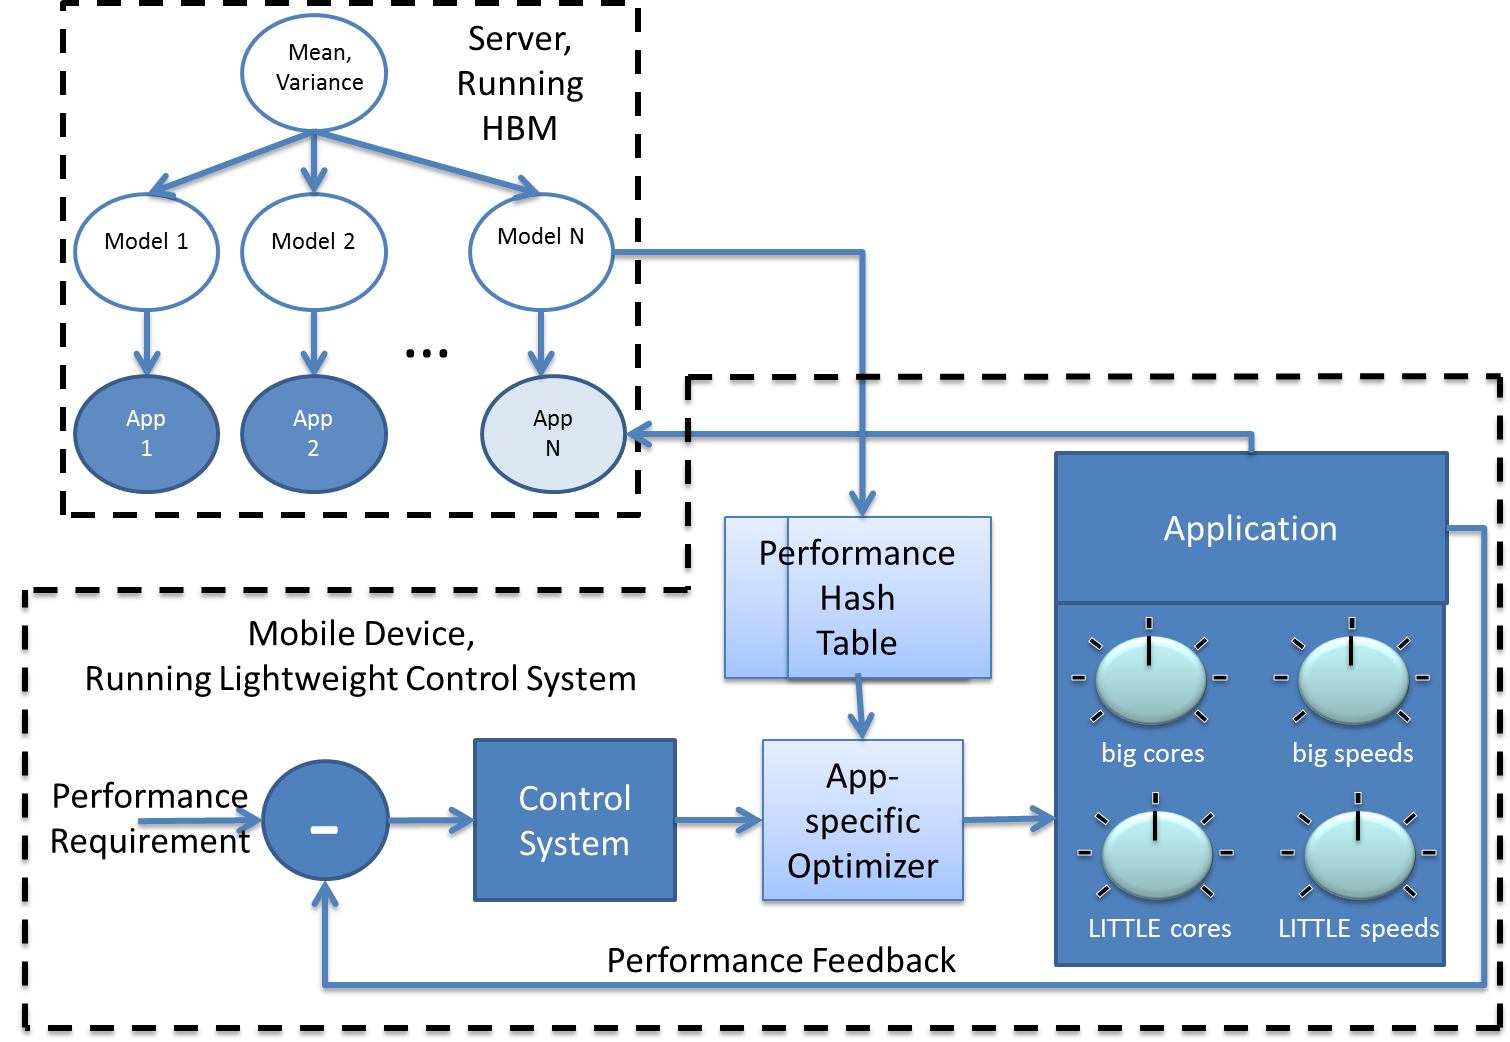
\includegraphics[width=\columnwidth]{figures/ControlLearning.png}
% \caption{\SYSTEM{} overview. A remote HBM generates a model, stored in
%   the performance hash table, which is used to control resources to
%   meet a performance goal for an application running on a
%   heterogeneous mobile system.}
%   \label{fig:overview}
% \end{figure}
\label{sec:framework}

%Overview. Learning background.  Control background.
\SYSTEM{} combines learning with control to tackle the complexity and
dynamics of modern mobile systems.  \figref{fig:overview} shows a detailed
overview of \SYSTEM{}.  A mobile system runs an application and some small number of performance measurements
are taken on a device and sent over to a server.  The server uses a
hierarchical Bayesian model to combine these measurements with ones
taken on other devices and with measurements of other applications. \SYSTEM{} uses an HBM based on LEO, a learning system build to
estimate application performance and power for server systems
\cite{LEO}.  LEO originally ran on the system to be optimized, but it
is far too computationally expensive to be run on a mobile phone --
even on the server for which it was designed, LEO has high overhead.
In \SYSTEM{}, we configure LEO to run as a remote server, to build
models of other systems based on data it is sent. Using this large volume of data, the HBM produces a model of
performance and power for all combinations of resources on the device.
On the mobile device, this model is stored in a novel data structure, called a
\emph{performance hash table} (PHT), which is the key interface
between the remote HBM and the lightweight control system (LCS) that
manages the device.  The LCS adjusts resource usage to meet
performance requirements for interactive mobile applications with
minimal energy.  The PHT is the key data structure allowing the LCS to
apply the learned models in constant ($O(1)$) time.  
%Producing the PHT is significantly more expensive, but it is done remotely and does not impact the device to be managed.  
In this manner, the HBM handles the
complexity of the device and the LCS handles the dynamics, with the
PHT being the key interface linking the two.  This section provides a
brief overview of the relevant learning and control techniques used in
\SYSTEM{}, and then describes the interface that combines them.

\subsection{Hierarchical Bayesian Learning}
\label{sec:framework:HBM}

%\PUNT{
\begin{figure}

  \subfloat[]
  {
    %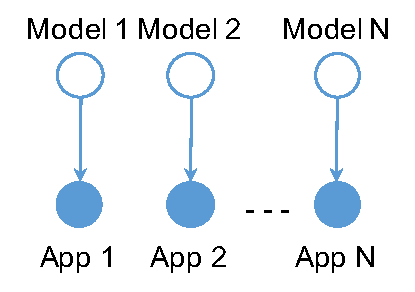
\includegraphics[width=.33\textwidth]{figures/Online.pdf}
    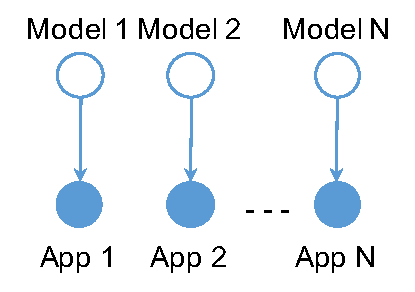
\includegraphics[width=.33\columnwidth]{figures/Online.pdf}

    \label{fig:online}
  }
  \subfloat[]
  {
    %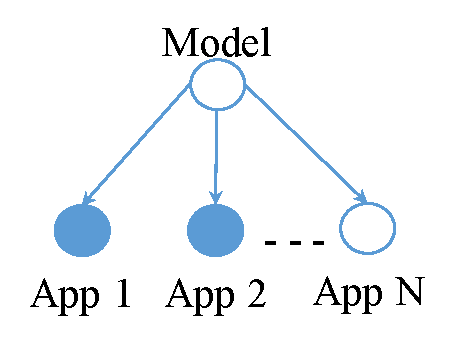
\includegraphics[width=.33\textwidth]{figures/Offline.pdf}
    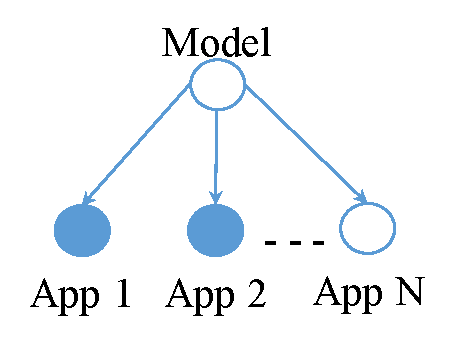
\includegraphics[width=.33\columnwidth]{figures/Offline.pdf}

    \label{fig:offline}
  }
  \subfloat[]
  {
    %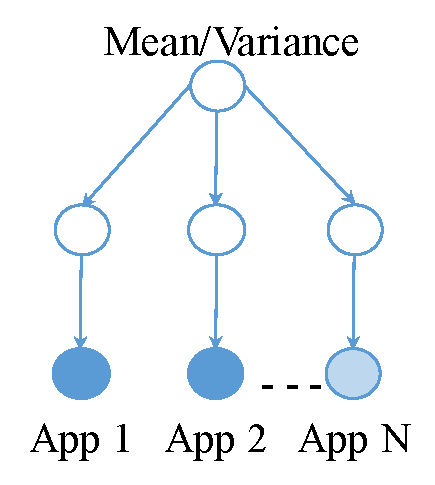
\includegraphics[width=.33\textwidth]{figures/HBM.pdf}
    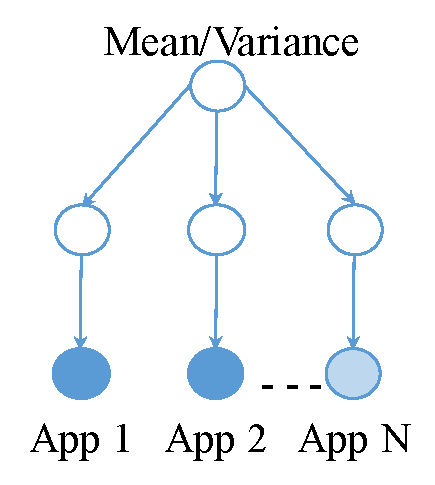
\includegraphics[width=.33\columnwidth]{figures/HBM.pdf}

    \label{fig:HBM}
  }
  \caption{ Comparison of online (a) offline (b) and hierarchical
    Bayesian models (c). The online model is concerned only with the
    current application (labeled N), the offline model combines all
    observations into one model, and the HBM builds per-application
    models, but makes them conditionally dependent on one another so
    that prior observations can be used to increase the accuracy of
    the model built for application N.}
\label{fig:learning-models}
\end{figure}
%}
\PUNT{
\begin{figure*}
   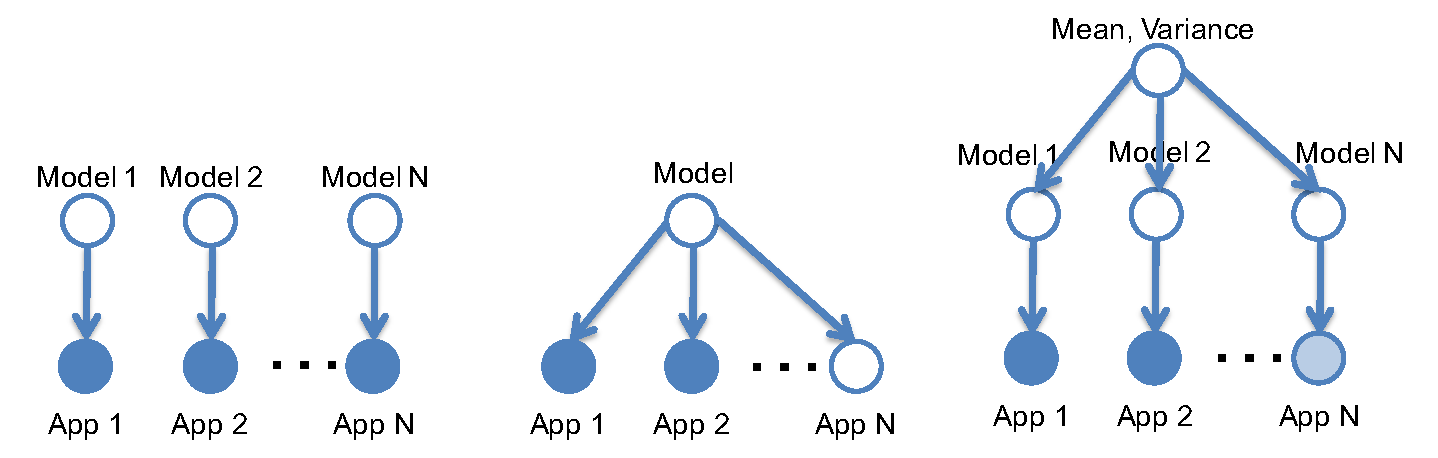
\includegraphics[width=\textwidth]{figures/online_offline_HBM.pdf}
   \caption{ Comparison of online, offline, and hierarchical Bayesian
     models.  The arrows represent dependences, circles are random
     variables, white circles are hidden variables that cannot be
     observed and must be learned, solid circles represent fully
     observed data, and shaded circles represent partially observed
     data.  The online model is concerned only with the current
     application (labeled N), the offline model combines all
     observations into one model, and the HBM builds per-application
     models, but makes them conditionally dependent on one another so
     that prior observations can be used to increase the accuracy of
     the model built for application N.}
\label{fig:learning-models}
\end{figure*}
}

Machine learning models are predictive in nature.  They take
observations of some phenomena and create a model to predict future
outcomes. In this work, we use a hierarchical Bayesian model (HBM) to
turn observations of applications' performance and power into
predictions about how other, unobserved resource allocations will
alter that performance and power.  We use a HBM because it provides a
statistically sound framework for learning across applications and
devices.  The HBM is non-parametric in terms of resource
configurations, hence well suited to learning the complicated
trade-off spaces that arise from heterogeneity in modern mobile
processors, like those illustrated in \figref{fig:lavamd_contour} and \figref{fig:kmeans_contour}.  This
non-smoothness is the reason why parametric models based on
clockspeed/cores of these curves do not perform well and the
hierarchical Bayesian model -- which is non-parametric -- is not
affected by the shape of the curve. \TODO{We still need one or two
  sentences to explain what this means and why it is good.}
%Online Models

%Offline Models

%HBM

%\TODO{I am not sure it is clear how learning addresses complexity.}


%This HBM-based learner runs
%on a remote server (originally in LEO it ran natively on the system to
%be optimized).

We compare \SYSTEM{} to an \emph{online model}, which only uses only
observations of the current application.  For such model to be
predictive, it must be parametric in terms of the configuration space
(cores/clockspeed) since no other information is available. This
online model requires a certain number of samples to estimate the
model parameters with low error.  Unfortunately, the model might still
falter if the model parameterization is not correct; \eg{} if the model
is misspecified and defined to be linear in cores, but the application
actually hits an asymptote and no longer increases performance after
some core count.

We also compare \SYSTEM{} to a purely \emph{offline model} which only
uses information from previously seen applications but lacks any
knowledge of the current application to be optimized. This general
model will capture trends; \eg{} when most applications should
transition from LITTLE to big cores, but it might miss the key
inflection point for some applications.

The HBM provides a good balance between the online and offline
approaches.  The key differences between these three approaches are
illustrated in \figref{fig:learning-models}. In this figure, circles
represent random variables, directed edges show conditionally
dependent relationships, and shading represents observability.  A dark
circle means we have seen all the data, a shaded circle means we have
some partial observations, and the white circle means that the
variable is unobservable.  The models we are trying to learn
are unobservable.  A strictly online approach will handle each new
application completely separately and ignore observations of previous
applications.  This approach never risks contaminating a model with
unrelated observations, but it may take many observations of the
current application to converge because it starts with no prior
knowledge. The offline approach uses all observations from prior
applications and will therefore converge very quickly; however, it is
overly general and cannot learn features specific to a single
application.
%%
\PUNT{
When selecting a learning framework we must find a trade-off between
the specific and the general; \ie{} between frameworks that build
application-specific models and frameworks that combine observations
across applications.  For example, the key to energy efficiency on
heterogeneous mobile systems is knowing when to make use of the
smaller, low-power cores \cite{reddiHPCA2013,POET}.  An
application-specific model will capture that precisely, but may
require many observations before producing the correct model.  A more
general model will capture the trend, \eg{} when most applications
should transition, but this general model might miss the key
inflection point for some applications.  We refer to
application-specific models as \emph{online} because they build models
for the current application and do not incorporate knowledge of other
applications.  We refer to general models as \emph{offline} as they
use prior observations of other applications to predict the behavior
of a new application.
}


The HBM (illustrated in \figref{fig:HBM}) is a superior combination of the
above discussed approaches (\emph{online} and \emph{offline}). The
model benefits from both (1) observations of the current application
and (2) the previously observed applications.  The model relies on
accurately learning the correlations between different configurations
based on the data from previously seen applications. Since, dimension
of the model's parameter, the correlation matrix scales with the
number of configurations the model is non-parametric.  Unlike an
\emph{offline} scenario, here each application has its own model,
allowing specificity, but these models are conditionally dependent on
some underlying probability distribution with a hidden mean and
co-variance matrix. In practice, the HBM will estimate a model for a
new application using a small number of observations of that
application (possibly from different devices) and combining those
observations with many prior observations of other applications. This
method generates a new model for the new application, which most
agrees with the learned correlations and the new samples in hand.
Rather than over-generalizing, the HBM implicitly uses similar
applications to produce new models.  In addition, the HBM's accuracy
increases as more applications are observed because more different
types of behavior are represented in the pool of prior knowledge.  Of
course, the computational complexity of learning -- which is linear in
the number of applications -- also increases with increasing
applications, but this is why we offload the learning to a remote
server.

\PUNT{
To provide intuition we offer a simple example.  Suppose we have
observed many prior applications, all of which are either completely
compute-bound or completely memory-bound, and we have an equal number
of both.  The only resource we can allocate is clockspeed, which will
increase the performance of compute-bound applications, but not
memory-bound ones.  When we need to work with a new application, we
need to estimate its response to clockspeed.  The online model will
not use prior knowledge, but will observe many different clock speeds
for the new application, leading to high overhead.  The offline model
will predict the mean response of prior applications, meaning it will
over-allocate speed to memory-bound applications and under-allocate to
compute-bound ones.  The HBM will take a small number of observations
and then the prediction will combine those with prior knowledge: if
the new observations show that clockspeed has little effect on
performance the HBM will use only the prior memory bound applications
to build its model, otherwise, it will use the compute-bound
applications.  In practice, the HBM learns much more complicated
relationships by combining observations of the new application with
prior knowledge of different types of behavior.
}



% We test LEO's accuracy compared to existing online and offline
% approaches to is 13.4\% better than online and 19.1\% better than
% offline in terms of performance estimation and LEO is 3.7\% better
% than online and 1.5\% better than offline in terms of power
% estimation, on average over all the benchmarks.

\subsection{Controlling Computing Systems}

Control theory provides a discipline for tuning parameters to ensure
that a system meets some requirement in a dynamic environment.  We use
a controller to meet a performance goal (corresponding to a
quality-of-service or real-time constraint) and adjust system resource
usage to see that the goal is met.  Our primary concern is making a
control formulation that is general enough to be applied to a wide
range of possible applications while receiving its model from the HBM.

We would like to use control and learning to solve the problem of
meeting an application's performance requirements while minimizing
energy consumption.  The difficulty is that classical control
formulations integrate the models directly into the controller; \ie{}
the application-dependent relationship between performance and the
controlled resource is directly used in the control equations.  For
example, consider a control system designed to meet a performance goal
by managing processor frequency.  This controller's coefficients would
directly encode the relationship between frequency and application
performance.  On mobile devices, we need to capture the relationship
between all available resources and application performance, but this
relationship is obviously application specific.  Thus, we face the
problem of implementing a general control system that is applicable to
a number of applications, and where the models relating resources to
performance are not known ahead of time.

We propose to address this problem using the classic computer science
trick of adding a layer of indirection.  This idea is illustrated in
\figref{fig:overview}.  Instead of directly controlling resources using an
application-dependent model, we will control \emph{speedup} and pass
that speedup value to a separate module that optimizes energy while
respecting this speedup constraint using the learned models.  Similar
models have been used to build generalized controllers where users are
responsible for supplying the models \cite{POET}.  Our goal is to
eliminate this user burden and have a remote HBM supply the model, which are not just more accurate but become more intelligent with time as it acquires more data.

\subsubsection{Controlling Speedup}
We write a simple difference model relating speedup to performance:
\begin{equation}
  perf(t) = m \cdot speedup(t-1) + \delta \label{eqn:speedup}
\end{equation}
where $m$ is the \emph{max speed} of the application, here defined as
the speed when all resources are available.  While $m$ is application
specific, it is easy to measure online, by simply allocating all
resources. Such a configuration should not violate any performance
constraints (although it is unlikely to be energy efficient) so it is
safe to take this measurement without risk of violating performance
constraints.

With this model, the control law is simply:
\begin{eqnarray}
  error(t) &=& goal - perf(t) \label{eqn:speedup-error} \\
  speedup(t) &=& speedup(t-1) - \frac{error(t)}{m}
  \label{eqn:speedup-control}
\end{eqnarray}
which states that the speedup to apply at time $t$ is a function of
the previous speedup, the error at time $t$ and the max speed $m$.
This is a very simple \emph{deadbeat} controller that provides all the
standard control theoretic formal guarantees
\cite{seec-cdc2010,ICSE2014}.  By measuring max speed online while the
application runs, we can tune the control to a specific application.
Using this definition of max speed, most speedups will be less than
one.  In addition to making max speed easier to measure, this has the
nice property of bounding the learner's output, making for more robust
learning \TODO{Nikita, what am I trying to say here? Or should we just
  put a forward reference because the next section benefits from a max
  speedup of 1} Of course, we still have the challenging problem of
converting an abstract speedup into an actual resource allocation.


\subsubsection{Optimizing Speedup}
We need to map the speedup produced by \eqnref{speedup-control} into a
resource allocation.  On our target system, an ARM big.LITTLE
architecture, that specifically means mapping speedup into a number of
big cores, a number of small cores, and a speed for both (on our
system big and little cores can be clocked separately).

The primary challenge here is that the HBM produces a non-linear
function mapping discrete resource allocations into speedup and
powerup, while \eqnref{speedup-control} is a continuous linear
function.  We bridge this divide by assigning time to resource
allocations such that the average speedup over a control interval is
that produced by \eqnref{speedup-control}.

We call an assignment of time to resources a \emph{schedule}. We call
a combination of settings for each resource a \emph{configuration}.  For
example, using two big cores at 1.5 \GHz and putting all the little
cores to sleep is one configuration.  Not surprisingly, there are
typically many schedules that meet a particular performance
requirement.  To extend battery life, we would like to find a minimal
energy schedule. Given a time interval $\tau$, a workload $W$ to
complete in that interval, and a set of $C$ configuration, we
formalize this problem as:
\begin{eqnarray}
  \minimize && \sum_{c=0}^{C-1} \tau_c \cdot p_c \label{eqn:power} \\
  \st %&& \nonumber\\
  && \sum_{c=0}^{C-1} \tau_c \cdot s_c \cdot b =  W \label{eqn:work} \\
  && \sum_{c=0}^{C-1} \tau_c =  \tau \label{eqn:deadline} \\
  && 0 \le \tau_c \le \tau, \qquad \forall c \in \{0,\ldots,C-1\} \label{eqn:time}
\end{eqnarray}
where $p_c$ and $s_c$ are the estimated powerup and speedup of
configuration $c$ and $\tau_c$ is the amount of time to spend in
configuration $c$.  \eqnref{power} simply states that the objective is
to minimize energy (power times time).  \eqnref{work} states that the
work must be done, while \eqnref{deadline} requires the work to be
done on time.  \eqnref{time} simply avoids negative time.  


\subsubsection{A Fast Algorithm For Resource Scheduling}
While most linear programming problems would be inefficient to solve
repeatedly on a mobile device, the one in \eqnrref{power}{time} has a
constant time ($O(1)$ solution.  Kim et al. analyzed heuristic
solutions to the problem of minimizing energy while meeting a
performance constraint \cite{kim-cpsna}.  They observed that there
must be an optimal solution with the following properties:
\begin{itemize}
\item At most two of $\tau_c$ are non-zero, meaning that at most two
  resource configurations will be used in any time interval.  This
  property both drastically limits the search space and puts a limit
  on the overhead of switching configurations, since it is never
  profitable to switch more than twice in an interval.
\item If one plots the configurations in the power and performance
  tradeoff space (so that performance is on the x-axis and power is on
  the y-axis) the two configurations with non-zero $\tau_c$ lie on the
  lower convex hull of the power performance tradeoff space.
\end{itemize}
We use these two facts to construct a constant time algorithm for
finding the optimal solution to \eqnrref{power}{time} online.  The
intuition behind our solution is illustrated in the upper half of
\figref{fig:pht}.  This figure shows a hypothetical example of the power
and performance tradeoffs the HBM might learn for some application and
device.  Each point represents a configuration and each configuration
is charted with normalized performance on the x-axis and normalized
power on the y-axis.  For any feasible performance requirement, there
is a minimal energy schedule that uses no more than two of the
configurations on the lower convex hull as any points that lie above
the lower convex hull require more power for equivalent performance
\cite{kim-cpsna}.  Therefore, the HBM estimates the power and
performance of all configurations, then finds the lower convex hull,
and sends that to the LCS.  The lower convex hull is the interface
between the HBM and the LCS, and the key enabler of \SYSTEM{}'s
combination of learning and control.

% \begin{figure}
% 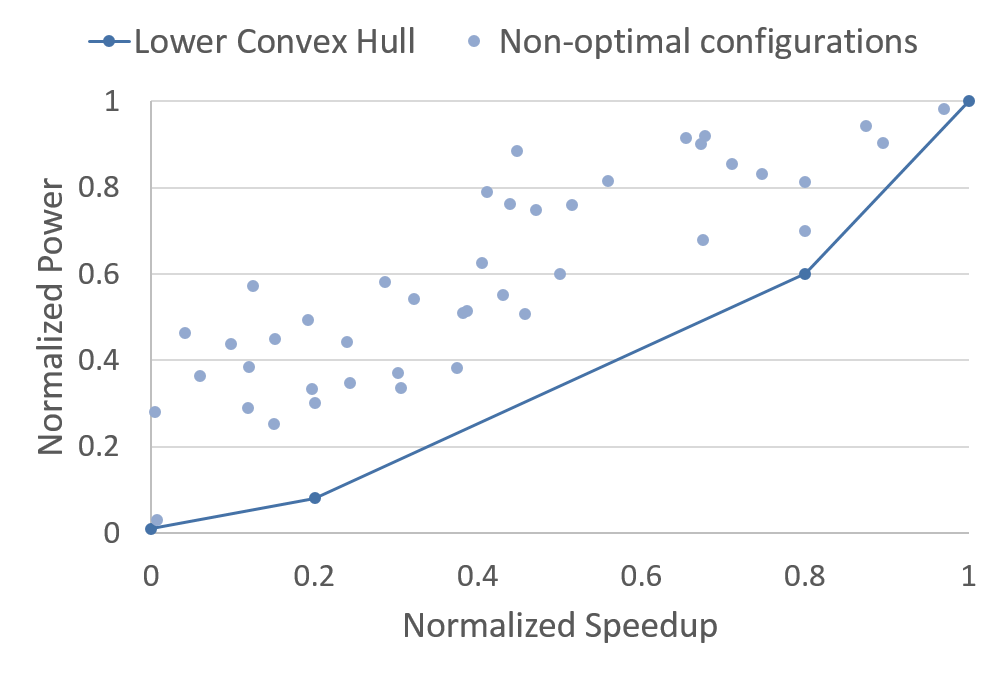
\includegraphics[width=\columnwidth]{figures/TradeoffExample.png}
% \caption{Example of plotting configurations in the power versus
%   performance space.}
%   \label{fig:convexhull}
% \end{figure}



\begin{figure}
  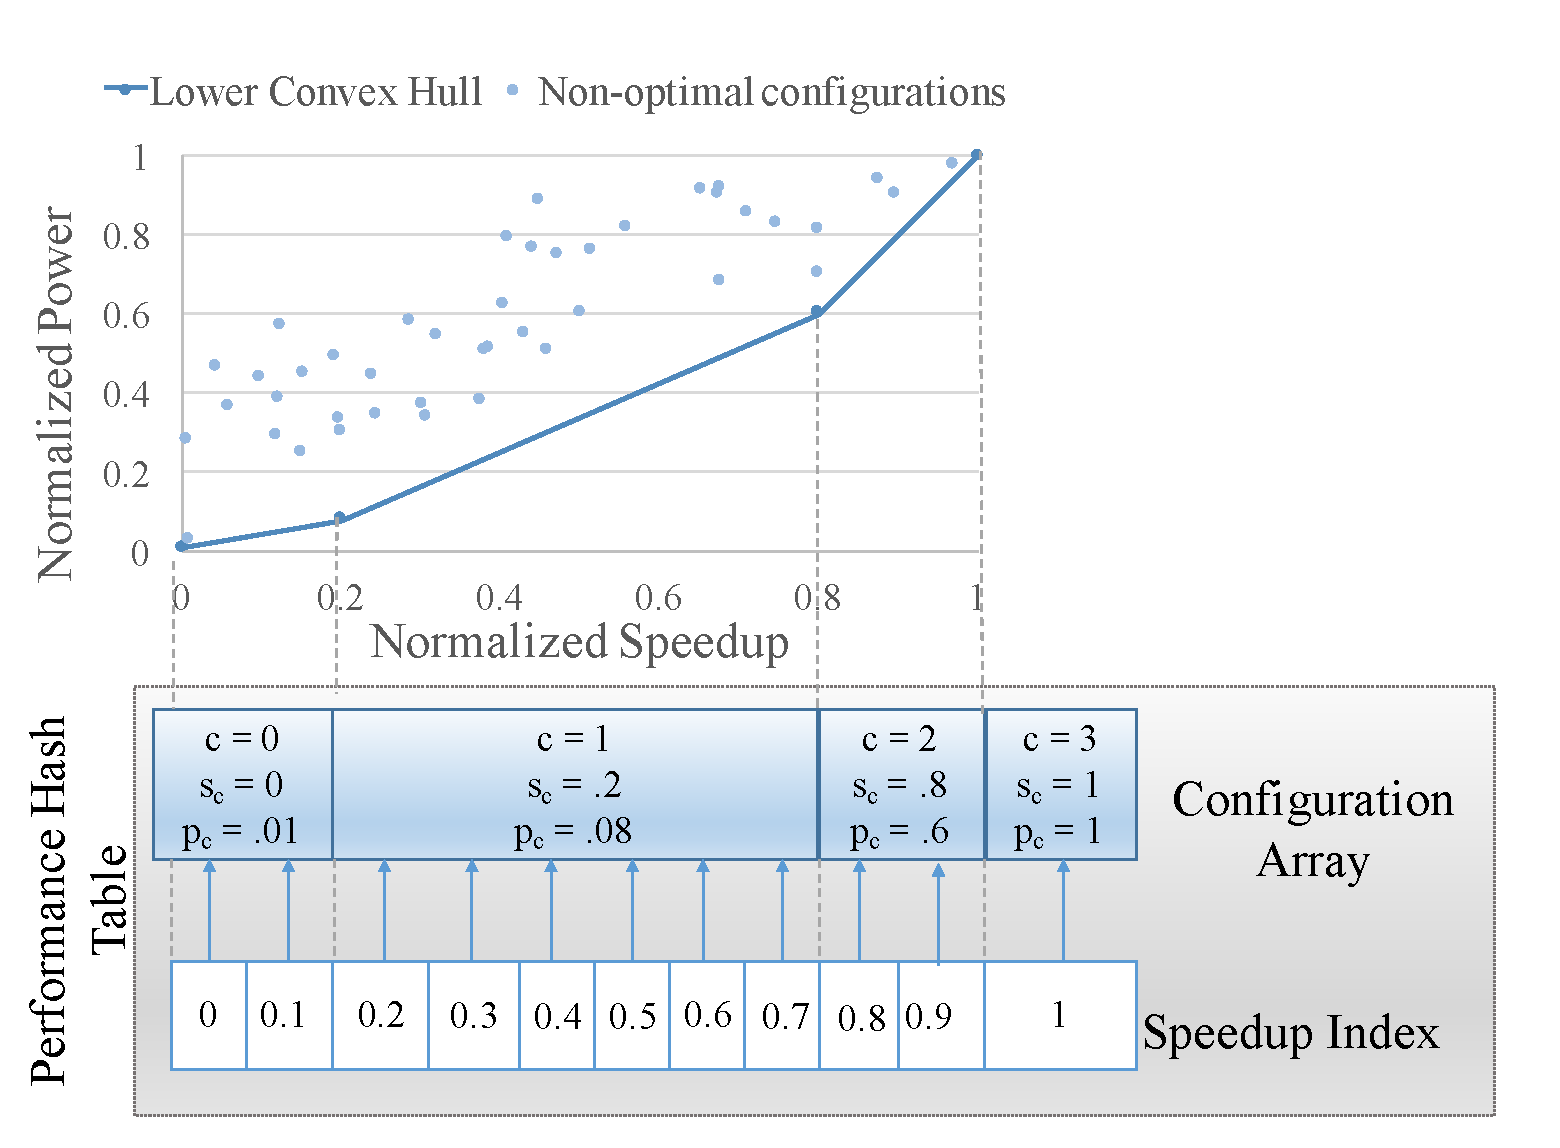
\includegraphics[width=\columnwidth]{figures/performance-hash-table.pdf}
  \caption{The Performance Hash Table and its relationship to the
    configuration space.  The HBM encodes the configuration as the
    lower convex hull of points in the performance/power tradeoff
    space and stores those in a table indexed by speedup.}
  \label{fig:pht}
\end{figure}

The HBM stores the lower convex hull in a \emph{performance hash
  table} (PHT).  The PHT and its relationship to the lower convex hull
is illustrated in \figref{fig:pht}.  It consists of two arrays, the first
is an array of pointers into the second array, which stores the
configurations on the lower convex hull sorted by speedup.  Recall
that speedups are computed relative to the maximum speed.  We
therefore know the largest speedup is 1, so we need only concern
ourselves with speedups less than 1.  The first table of pointers has
a \emph{resolution} indicating how many decimal points of precision it
captures.  The example in \figref{fig:pht} has a resolution of $0.1$.
Each pointer in the bottom  table points to the configuration in the
second array that has the largest speedup less than or equal to the
index.

To use the table, the optimizer receives a speedup $s(t)$ from the
controller.  It needs to convert this into two configurations referred
to as $hi$ and $lo$.  To find the $hi$ configuration, the optimizer
clamps the desired speedup to the largest index lower than $s(t)$ and
then walks forward until it finds the first configuration with a
speedup higher than $s(t)$.  To find the $lo$ configuration, the
optimizer clamps the desired speedup to the smallest index higher than
$s(t)$ and then walks backwards until it finds the configuration with
the largest speedup less than $s(t)$.

For example, consider the PHT in \figref{fig:pht} and an optimizer trying
to meet a speedup $s(t) = .65$.  To find $hi$, the optimizer indexes
at .6 and walks up to find $c=2$ with $s_c=.8$, setting $hi = 2$.  To
find $lo$, the optimizer indexes the table at .7 and walks backward to
find $c=1$ with $s_c=.2$, setting $lo = 1$.

Finally, the optimizer sets $\tau_{hi}$ and $\tau_{lo}$ by solving the
following set of equations:
\begin{eqnarray}
  \tau &=& \tau_{hi} + \tau_{lo}    \label{eqn:s1} \\
  s(t) &=& s_{hi} \cdot \tau_{hi} + s_{lo} \cdot \tau_{lo} \label{eqn:s2} 
\end{eqnarray}
In these equations, $s(t)$ is the speedup requested by the optimizer
and $s_c$ are speedups estimated by the learner.

By solving \eqnsref{s1}{s2}, the optimizer has turned the controller's
requested speedup into a schedule of resource allocations using the
models provided by the HBM.  Provided that the resolution is large
enough to get a good spread of configurations to indices, the
optimizer will always index the configuration array at most one entry
from where it needs to be.  Thus, the entire optimization process runs
in constant time -- assuming that the learner is responsible for
building the PHT once before passing it on to the optimizer.  This
efficiency comes at a cost of memory usage, as many of the entries in
the speedup index table will point to redundant locations in the
configuration array.  This tradeoff is reasonable in practice as the
code that runs on the mobile device must be fast or we risk wasting
energy while trying to save energy.  In practice, we recommend a table
of size 100 which provides a sufficient resolution and is not too
wasteful of space.

\PUNT{
\subsection{Putting It All Together}
We briefly summarize our proposal for combining learning and control.
Our approach consists of a number of independent mobile devices each
running a lightweight controller.  Each device makes a small number of
local observations of an application it runs and sends those to the
server.  The server integrates those observations in its HBM to
produce customized models for each device.  These models are sent back
to the individual devices where they are used to meet performance
requirements with minimal energy by turning a speedup signal into an
optimal schedule of configurations.

\TODO{The control theoretic guarantees are still valid provided that
  the error in the learned speedup is not too great.  Is it worth
  analyzing those formal guarantees?}

}

%control slowdown

%map slowdown into configurations

% solve optimization problem

% slowdown table

